\section{投影与最近点：从一条直线走向一般子空间}
\label{sec:03-Linear-Algebra/03-Orthogonality/02}

一张手抄的账单上写着三个数：两笔小计和一个总额，以百元计，
\[
c=(2,\;1,\;4)^{\trans}.
\]
可是 \(2+1\neq4\)。总额本该等于两笔小计之和，这条约束把所有``自洽的账单''限制在一个二维平面上——\(\R^3\) 中满足 \(c_3=c_1+c_2\) 的全部向量。手上这一张不在平面里。

你不打算推翻整张单子，只想改得尽量少。于是问题成形了：在那个平面上，哪一点离 \(c\) 最近？

这不是账房先生独有的问题。用直线拟合散点、用低维子空间压缩数据、在控制中挑一个最接近目标的可达状态，都是同一个模板换了场景——目标 \(b\) 给定，能力受限的模型只覆盖子空间 \(S\)，求 \(S\) 中离 \(b\) 最近的那一点。上一节已经证明 \(b\) 能唯一分解成 \(S\) 内的一段加上 \(S^{\perp}\) 内的一段，本节把这个分解算出来，顺带说清那一段为什么就是最近点。

\subsection{一条直线上的垂足给出全部逻辑}

设非零向量 \(a\) 张成直线 \(S=\operatorname{span}\{a\}\)。直线上的点都写作 \(p=\hat x a\)，\(\hat x\) 是待定标量。若 \(p\) 是最近点，残差 \(e=b-\hat xa\) 就必须与直线垂直——否则 \(e\) 在 \(a\) 方向上还留着分量，顺着那个方向微调 \(\hat x\)，距离还能再短一点。于是 \(a^{\trans}(b-\hat xa)=0\)，解出
\[
\hat x=\frac{a^{\trans}b}{a^{\trans}a},
\qquad
p=a\,\frac{a^{\trans}b}{a^{\trans}a} .
\]
两个量不能混：\(\hat x\) 是基向量前面的系数，是个标量；而 \(p\) 才是落在 \(\R^m\) 里的投影向量。把系数当成投影本身，推广到高维时会立刻撞上维度不匹配。

拿 \(b=(2,0)^{\trans}\) 投到 \(a=(1,1)^{\trans}\) 张成的直线上：\(\hat x=2/2=1\)，\(p=(1,1)^{\trans}\)，\(e=(1,-1)^{\trans}\)，而 \(a^{\trans}e=0\)。

\begin{center}
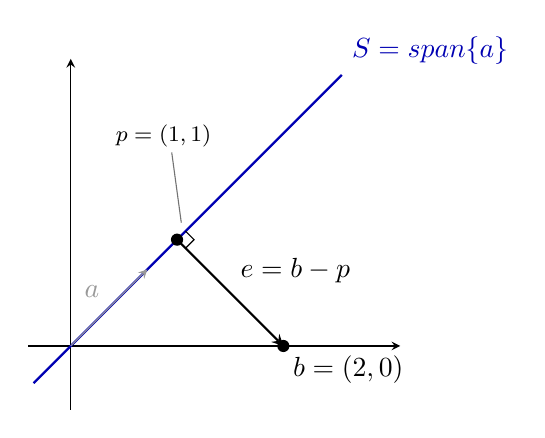
\begin{tikzpicture}[x=1.35cm,y=1.35cm,>=stealth]
  \draw[->] (-0.4,0) -- (3.1,0);
  \draw[->] (0,-0.6) -- (0,2.7);
  \draw[blue!70!black,thick] (-0.35,-0.35) -- (2.55,2.55)
    node[above right] {\(S=\operatorname{span}\{a\}\)};
  \fill (2,0) circle (2.2pt) node[below right] {\(b=(2,0)^{\trans}\)};
  \fill (1,1) circle (2.2pt);
  \node[font=\footnotesize] at (0.88,1.98) {\(p=(1,1)^{\trans}\)};
  \draw[black!55] (0.95,1.82) -- (1.04,1.16);
  \draw[->,thick] (1,1) -- (2,0) node[midway,above right] {\(e=b-p\)};
  \draw (1.08,0.92) -- (1.16,1) -- (1.08,1.08);
  \draw[->,gray!80] (0,0) -- (0.72,0.72) node[midway,above left] {\(a\)};
\end{tikzpicture}

\emph{投影 \(p\) 留在可行子空间中，残差 \(e\) 则落在正交补中；两者相加还原 \(b\)。}
\end{center}

图上那个小直角标记是这一节唯一的输入。剩下的全部内容，都是把它写成越来越一般的代数形式。

\subsection{垂足是唯一最近点，勾股定理直接给出}

为什么垂足就是最近点？勾股定理一步就给出答案，而且这个答案对``直线''的依赖只是表面现象。取直线上另一点 \(w=p+s\)，其中 \(s\in S\)。因为 \(e=b-p\) 属于 \(S^{\perp}\)，所以 \(e\perp s\)，于是
\[
\begin{aligned}
\norm{b-w}_2^2
&=\norm{e-s}_2^2\\
&=\norm{e}_2^2+\norm{s}_2^2\\
&\ge\norm{e}_2^2 ,
\end{aligned}
\]
等号只在 \(s=0\)、也就是 \(w=p\) 时成立。

这段推导里没有一处用到``直线''。用到的只有 \(p\in S\)、\(e\in S^{\perp}\) 和勾股分解，所以它对任何子空间都成立：残差一旦垂直于整个子空间，\(p\) 就是唯一最近点。找最近点因此等价于找上一节那个正交分解 \(b=p+e\)。

\subsection{把垂直条件写成方程，就得到正规方程}

垂足的存在与唯一已经有了，剩下的是把它算出来——办法是把``垂直''这个几何条件翻译成代数方程。让子空间由矩阵的列张成，\(S=\operatorname{Col}(A)\)。候选向量形如 \(p=A\hat x\)。残差要垂直于整个列空间，等价于垂直于每一列，而 \(n\) 个垂直条件可以一次性打包：
\[
A^{\trans}(b-A\hat x)=0
\quad\Longrightarrow\quad
A^{\trans}A\hat x=A^{\trans}b .
\]
这就是正规方程。名字很正式，来路却只有一句话：残差与所有可行方向正交。\(A^{\trans}\) 在这里的职责就是把那些垂直条件收集成一个 \(n\times n\) 的对称系统。

若 \(A\) 的列线性无关，\(A^{\trans}A\) 可逆。理由很短：由 \(A^{\trans}Ax=0\) 左乘 \(x^{\trans}\) 得 \(\norm{Ax}_2^2=0\)，故 \(Ax=0\)，列无关又逼出 \(x=0\)；方阵的零空间平凡即可逆。于是
\[
\hat x=(A^{\trans}A)^{-1}A^{\trans}b,
\qquad
p=Pb,
\qquad
P=A(A^{\trans}A)^{-1}A^{\trans}.
\]

公式里每个因子都在做一次翻译。\(A^{\trans}\) 把``残差垂直于各列''收成 \(n\) 个条件，\((A^{\trans}A)^{-1}\) 在这些条件里解出最优坐标，最左边的 \(A\) 再把坐标还原成 \(\R^m\) 中的向量。三个向量 \(b,p,e\) 住在 \(\R^m\)，而坐标 \(\hat x\) 住在 \(\R^n\)，看清这一点就不会被公式的长相吓住。互补矩阵 \(I-P\) 做的是相反的事，\(e=(I-P)b\)；正交分解被这两个矩阵干净地一分为二。

\subsection{回到账单：改得最少的那张单子长什么样}

自洽账单构成的平面由
\[
A=\begin{pmatrix}1&0\\0&1\\1&1\end{pmatrix}
\]
的两列张成——任取 \(x,y\)，得到的向量就是 \((x,y,x+y)^{\trans}\)。代进公式，
\[
P=A(A^{\trans}A)^{-1}A^{\trans}
=\frac13\begin{pmatrix}2&-1&1\\-1&2&1\\1&1&2\end{pmatrix},
\qquad
Pc=\frac13\begin{pmatrix}7\\4\\11\end{pmatrix}.
\]
前两个分量之和 \(7/3+4/3=11/3\)，正是第三个分量：修改后的账单自洽了。残差 \(c-Pc=(-1,-1,1)^{\trans}/3\) 与 \(A\) 的两列都垂直，几何上就是开头那张图里的小直角，只不过子空间从直线换成了平面。

值得注意的是 \(P\) 与 \(c\) 无关。它是那个平面的属性，来一万张账单都用同一个矩阵去修。

不过修完之后要停下来想一想。这里给三处金额施加了相同的权重，因为用的是欧氏距离。可若总额抄自银行流水、两笔小计抄自便条，总额显然更可信，凭什么让它承担三分之一的改动？此时该换成加权距离，对不同分量施加不同惩罚，或者干脆把总额锁成硬约束、只优化小计。投影的``最近''永远是相对于某个内积而言的；数学保证公式正确执行，选哪把尺子仍然是你的判断。

\subsection{对称性才是正交投影的标志}

\(P\) 由公式唯一决定，于是可以反过来问：满足什么特征的矩阵才配叫正交投影？从公式可以直接读出两条性质：
\[
P^{\trans}=P,\qquad P^2=P .
\]
第一条用 \((M^{-1})^{\trans}=(M^{\trans})^{-1}\) 和 \(A^{\trans}A\) 的对称性一步得到；第二条只需注意中间的 \(A^{\trans}A(A^{\trans}A)^{-1}\) 化为单位阵。幂等的含义很直白——已经落在子空间里的向量，再投一次还是它自己。

麻烦在于反过来不成立：幂等推不出正交。矩阵
\[
M=\begin{pmatrix}1&-1\\0&0\end{pmatrix}
\]
满足 \(M^2=M\)，把任何向量送到 \(x\) 轴上，一次到位。可它把 \((0,2)^{\trans}\) 送去了 \((-2,0)^{\trans}\)，而 \(x\) 轴上离 \((0,2)^{\trans}\) 最近的点明明是原点。

\begin{center}
\begin{tikzpicture}[x=1cm,y=1cm,font=\small,>=stealth]
  \begin{scope}
    \draw[blue!70!black,thick] (-2.7,0) -- (2.7,0) node[right] {\(S\)};
    \fill (0,2) circle (2pt) node[above right] {\(b\)};
    \fill (0,0) circle (2pt) node[below left] {\(Pb\)};
    \draw[->,thick] (0,2) -- (0,0.07);
    \draw (0.22,0) -- (0.22,0.22) -- (0,0.22);
    \node at (0,-1.0) {正交投影：\(P^{\trans}=P\)};
  \end{scope}
  \begin{scope}[shift={(6.8,0)}]
    \draw[blue!70!black,thick] (-2.7,0) -- (2.7,0) node[right] {\(S\)};
    \fill (0,2) circle (2pt) node[above right] {\(b\)};
    \fill (-2,0) circle (2pt) node[below] {\(Mb\)};
    \draw[->,thick] (0,2) -- (-1.95,0.05);
    \draw[gray!60] (0,0) circle (3pt);
    \node[right,gray!60,font=\footnotesize] at (0.18,-0.42) {欧氏最近点在这里};
    \node at (0,-1.0) {斜投影：\(M^{2}=M\)，但 \(M^{\trans}\neq M\)};
  \end{scope}
\end{tikzpicture}

\emph{两种映射都满足``压一次就到位''，区别只在压的方向。左边沿垂直方向落下，残差与 \(S\) 成直角，落点是最近点；右边沿倾斜方向落下，落点偏出去一大截。对称性正是强制垂直方向的那个条件。}
\end{center}

所以在判断一个矩阵是不是正交投影时，两条都要查。只查幂等，斜投影会混进来；而斜投影虽然也是合法的投影，却不解决``最近''这个问题——它对应的是另一种分解方式，在斜坐标系或某些迭代格式里有用，但与本章的最小距离无关。

\subsection{列不满秩时，垂足还在，坐标散了}

\((A^{\trans}A)^{-1}\) 要求列线性无关。列一旦相关，比如两列完全相同，正规方程就有无穷多组解。但失效的东西必须说准：垂足 \(p\) 依然唯一，因为列空间是一个确定的子空间，最近点由几何决定，与你用哪组列去描述它无关。散掉的只是坐标——同一个 \(p\) 可以由无数种系数组合拼出来。

这个区分在数据工作里有个熟悉的名字。设计矩阵的两列若严格成比例，模型只依赖它们的某个组合，单个系数无从确定，统计上叫参数不可识别；两列若只是接近成比例，系数不再无穷多，却会变得极不稳定——共线性。预测值稳、系数乱，正是``垂足唯一、坐标不唯一''在有噪声时的连续版本。

出路有三条：删掉冗余列，重新用一个线性无关子集建模；为列空间造一组正交归一基，坐标改由点积直接读出；或者等学完 SVD 之后用伪逆，在\hyperref[sec:03-Linear-Algebra/07-SVD-and-Data-Applications/02]{``伪逆与病态问题''}里统一处理秩亏与近秩亏。第二条正是本章第四篇要走的路。

认出一个问题能写成``子空间中的最近点''，整套工具就直接可用了：线性回归、Fourier 级数截断、PCA 降维、Kalman 滤波的状态更新，都是同一个模板。变的只是子空间是什么、内积怎么选，公式的骨架不动。

下一节把这个模板套在最熟悉的场景上——用一条直线拟合三个点。你会看到回归系数的公式并不是某种统计学发明，它就是本节的 \(\hat x\)，只不过 \(A\) 的列换成了特征。
